\documentclass[a4paper,11pt]{article}
\usepackage{sobrapo-template}
\usepackage[brazil]{babel}
\usepackage[latin1]{inputenc}
\usepackage{amsmath,amssymb}

\usepackage{tikz}
\usetikzlibrary{calc}
\usetikzlibrary{shapes}
\usetikzlibrary{arrows}
\usetikzlibrary{backgrounds}

\usepackage[parfill]{parskip}

\newcommand{\NH}{\text{NH}}
\newcommand{\RG}{\text{RG}}

\title{An Incomplete Overview of some Applications of Game Theory to Patient Flow}

\begin{document}

\maketitle

\author{
\name{Vincent Knight}
\institute{Cardiff University}
\iaddress{Cardiff, UK}
\email{knightva@cf.ac.uk}
}

\author{
\name{Paul Harper}
\institute{Cardiff University}
\iaddress{Cardiff, UK}
\email{harper@cf.ac.uk}
}

\author{
\name{Jeff Griffiths}
\institute{Cardiff University}
\iaddress{Cardiff, UK}
\email{griffiths@cf.ac.uk}
}

\author{
\name{Izabela Komenda}
\institute{Cardiff University}
\iaddress{Cardiff, UK}
\email{komendai@cf.ac.uk}
}

\author{
\name{Rob Shone}
\institute{Cardiff University}
\iaddress{Cardiff, UK}
\email{shoner@cf.ac.uk}
}

\vspace{8mm}

\begin{abstract}
It is well observed that individual behaviour can have an effect on the efficiency of queueing systems.
The impact of this behaviour on the economic efficiency of public services is considered in this paper where we present results concerning the congestion related implications of decisions made by individuals when choosing between facilities.
The work presented has important managerial implications at a public policy level when considering the effect of allowing individuals to choose between providers.
We show that in general the introduction of choice in an already inefficient system will not have a negative effect.
Introducing choice in a system that copes with demand will have a negative effect.
\end{abstract}

\bigskip
\begin{keywords}
Patient Flow, Game Theory, Queueing Theory

\bigskip
\noindent{Main Area: Healthcare}
\end{keywords}


\newpage

\section{Introduction}

What damage do the selfish choices of some afflict on to the welfare of all? The work presented in this paper answers this question in the context of public service systems.

There is a substantial quantity of literature on the subject of equilibrium behaviour of a queueing system where congestion is a factor influencing behaviour \cite{Adler1969,Bell1983,Edelson1971,Knudsen1972,Luski1976,Naor1969,Yechiali1972}. This can be traced back to a series of short communications between Leeman \cite{Leeman1964,Leeman1965} and Saaty \cite{Saaty1965}. This paper builds on this literature by considering the problem of public service systems. For most public services, congestion is a negative aspect of service quality. Examples of this are healthcare systems (waiting lists), transports systems (traffic jams) and/or schools (overcrowding of class rooms).

The degree of central control that should be exercised is a very important question to be considered by governments and/or policy makers. What is the effect of allowing individuals to choose service provider?

Of course, the motivation for the introduction of choice is to create competition in the hope that this would improve overall service quality. The aim of the work presented here is to use a game theoretical approach to measure the immediate effect of choice (i.e. prior to the effect of competition). The approach proposed is based on a measure called \emph{the price of anarchy} \cite{Chau2003,Cole2006,Correa2008,Gilboa-Freedman2009,Haviv2007,Musacchio2009,Roughgarden2003,Roughgarden2005,Roughgarden2004,Skinner2010}. First introduced in \cite{Koutsoupias1999} (a conference paper that has been reprinted in \cite{Koutsoupias2009}), the price of anarchy is the ratio of the costs of the worst possible Nash equilibrium and the social optimum, and can therefore be interpreted as a measure of the efficiency of a system.

Game theory is the mathematical study of interactive decision making between rational decision makers \cite{Maschler2013}.
A game is a description of strategic interactions that includes the constraints on the actions that the players can take and on the players' interests.

Most research where game theory is applied in healthcare has mainly concentrated on Emergency Departments (EDs) and how to deal with diversions of patients and ambulances.
In \cite{Hagtvedt2009} cooperative strategies for hospitals are considered, in order to reduce occurrences when ambulances are turned away due to the ED being full.
In \cite{Deo2011} a queueing network model of two EDs is proposed to study the network effect of ambulance diversion.
Each ED aims to minimise the expected waiting time of its patients (walk-ins and ambulances) and chooses its diversion threshold based on the number of patients at its location. Decentralised decision making in the network is modelled as a non-cooperative game.

Some other work that has not concentrated on EDs, but has been applied to healthcare includes: \cite{Knight2013}, where results concerning the congestion related implications of decisions made by patients when choosing between healthcare facilities were presented. In \cite{Howard2002} a model of the accept/reject decision for transplant organs is developed.

In the wider intersection of game theory and queueing theory (where this work lies) papers that consider price and/or capacity include: \cite{Allon2007, Cachon2002,  Cachon2007, Kalai1992, Levhari1978}. In these models, the choice of price/or capacity determines the arrival rate for each firm; this is similar to the approach taken in this paper.


\section{Choosing queues}

This section describes how patient choices between various congestion affected services may be modelled.
In particular the situation shown diagrammatically in Figure \ref{fig:choices} is considered: patients have a choice amongst $M/M/c$ queues.

\begin{figure}[!hbtp]
\begin{center}
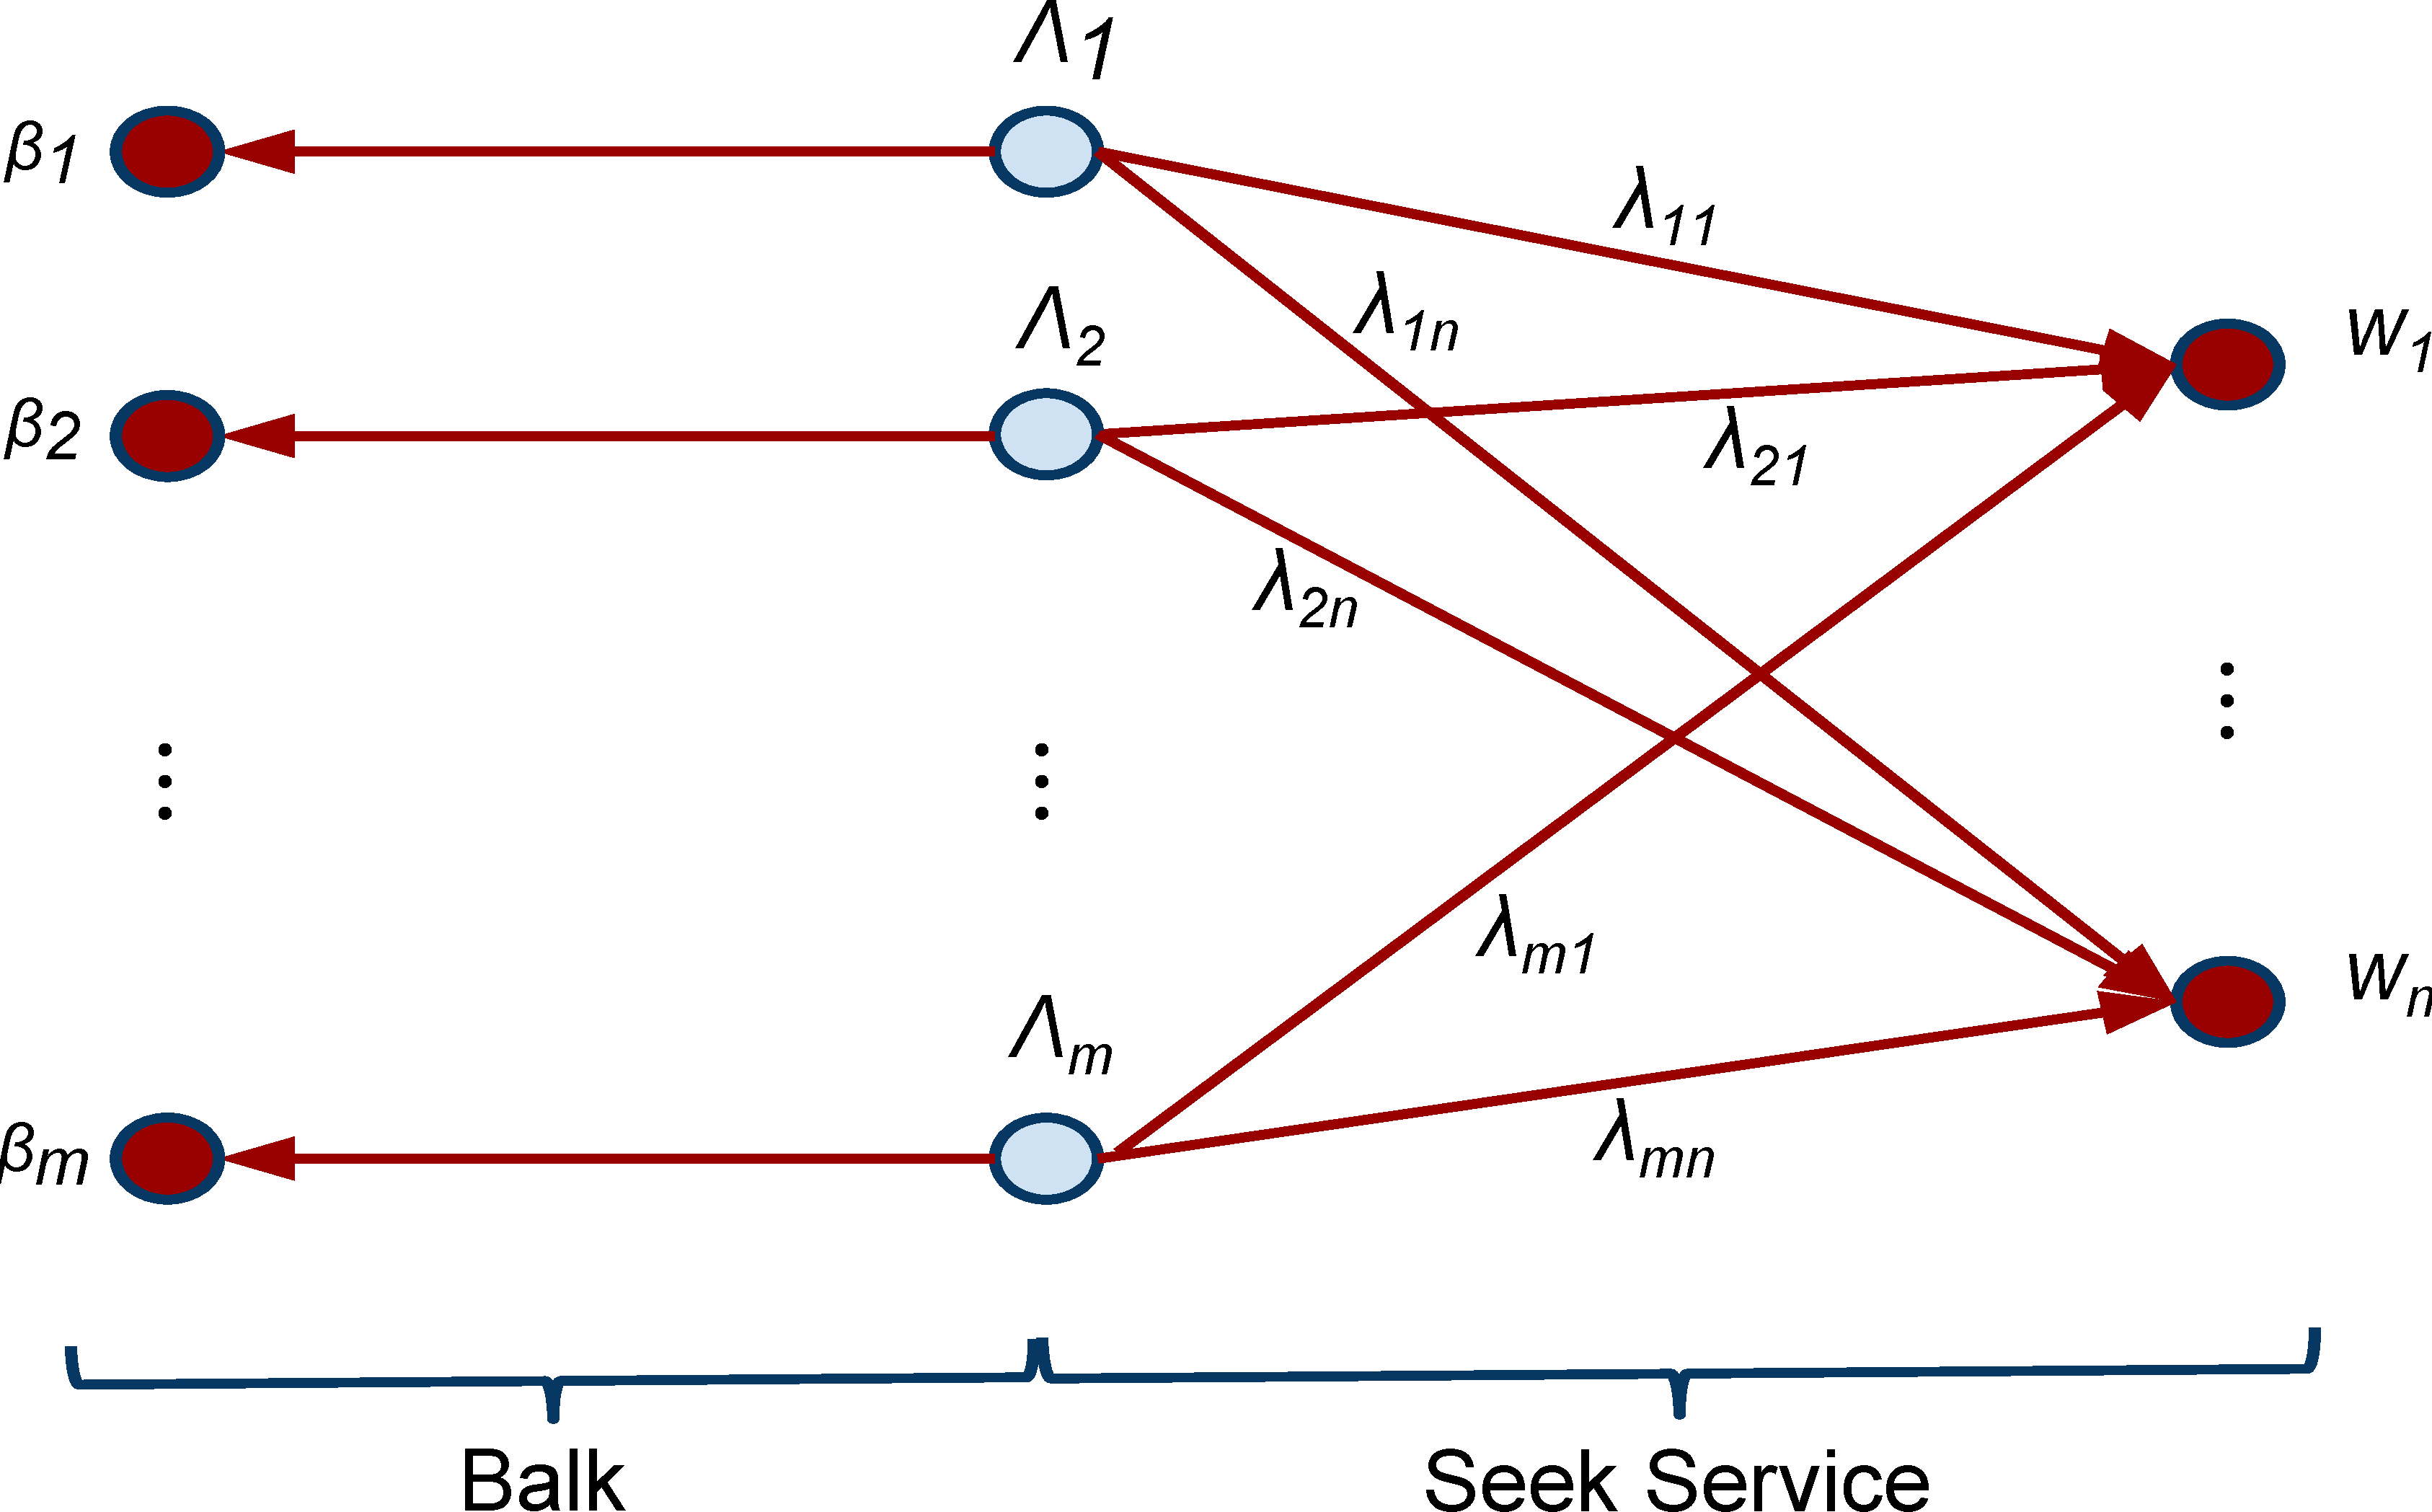
\includegraphics[width=.7\textwidth]{./Images/Hospital_Choices.pdf}
\end{center}
\caption{Routing patients from $m$ hospitals to $n$ services.}\label{fig:choices}
\end{figure}

There are two approaches to solving this problem: assuming that patients observe or not the system states before choosing a facility.
A rigorous comparison of these two approaches for individuals choosing to join an $M/M/1$ queue is given in \cite{}.

An unobservable study is given in \cite{} where routing games \cite{Rouhgharden} are used to study the system described.
The routing game used is shown in \ref{fig:routinggame}.

\begin{figure}[!hbtp]
\begin{center}
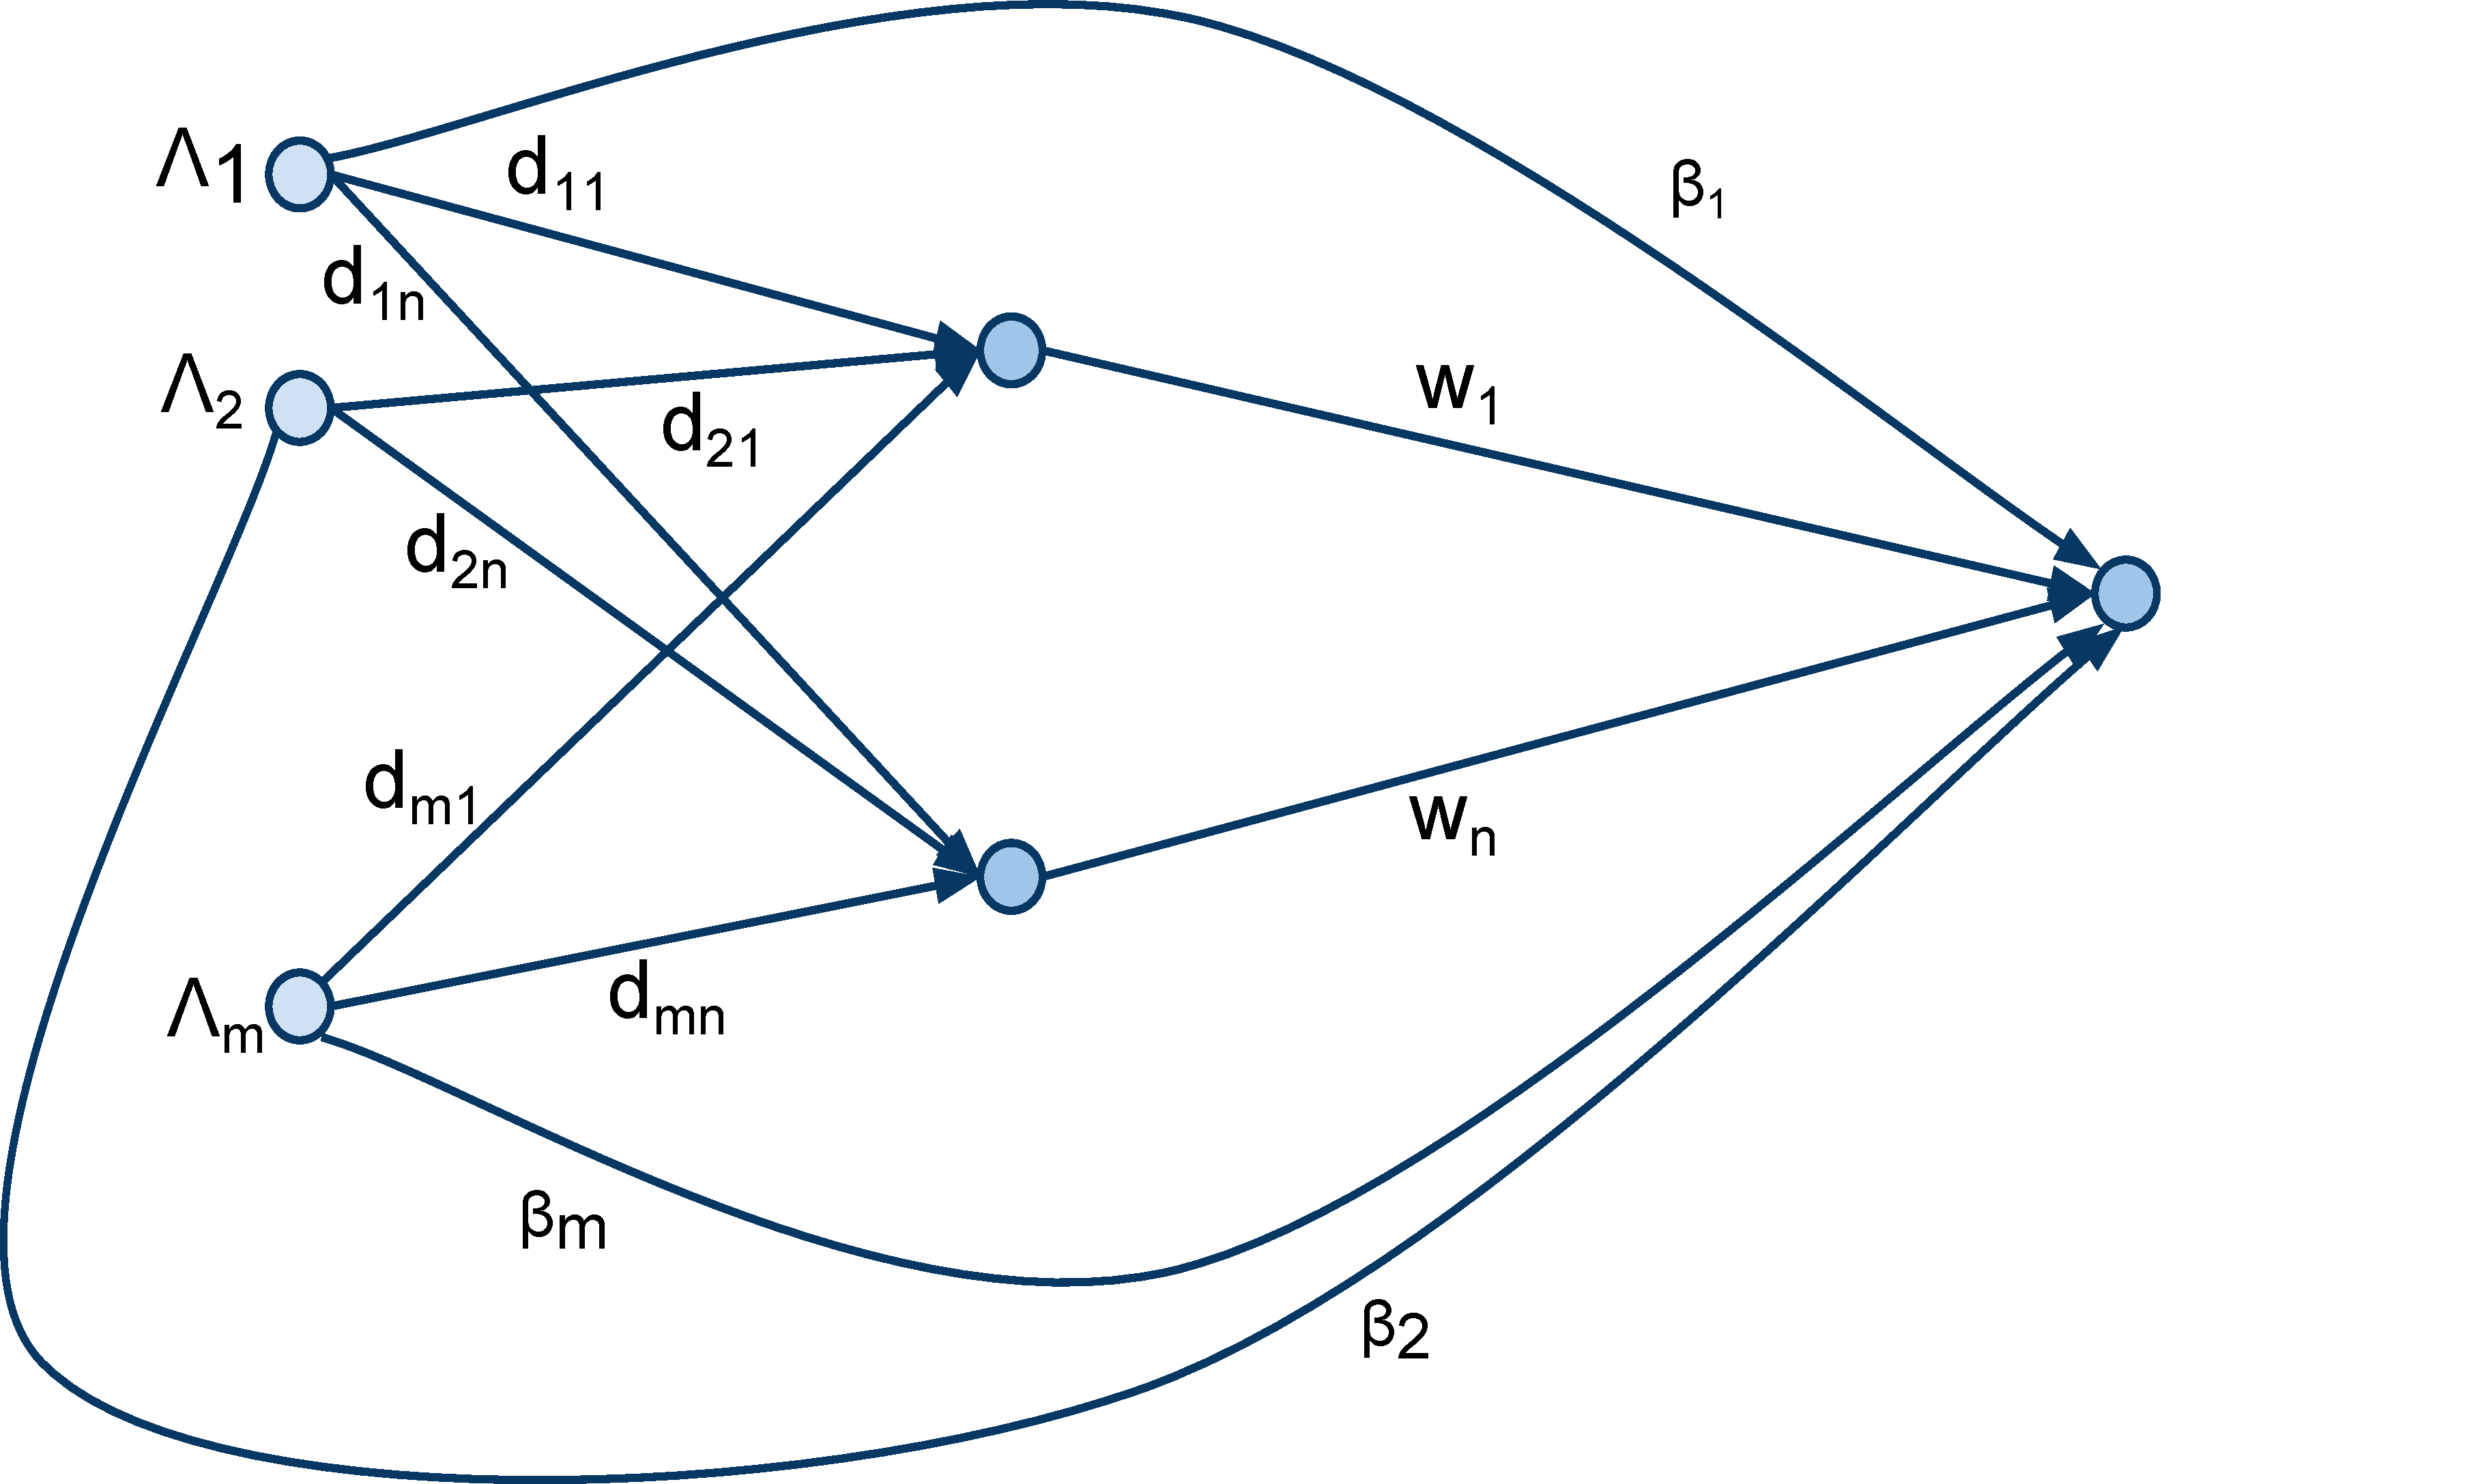
\includegraphics[width=.7\textwidth]{./Images/Hospital_Routing_Game.pdf}
\end{center}
\caption{Routing game $m$ hospitals to $n$ services.}\label{fig:routinggame}
\end{figure}

It can be shown that the cost for any given flow $\lambda$ (denoting the amount of traffic from source $i$ to facility $j$) corresponds to...

\begin{equation}
C(\lambda)=\sum_{i=1}^m\alpha_i\sum_{j}^nd_{ij}\lambda_{ij}+\sum_{j=1}^n\sum_{i=1}^m\lambda_{ij}w_j\left(\sum_{i=1}^m\lambda_{ij}\right)+\sum_{i=1}^m\beta_i\left(\Lambda_i-\sum_{j=1}^n\lambda_{ij}\right)
\label{C}\end{equation}

Obtaining the Nash flow: ie the equilibrium behaviour.

\begin{equation}
\Phi(\lambda)=\sum_{i=1}^m\alpha_i\sum_{j}^nd_{ij}\lambda_{ij}+\sum_{j=1}^n\int_0^{\sum_{i=1}^m\lambda_{ij}}w_j(x)dx+\sum_{i=1}^m\beta_i\left(\Lambda_i-\sum_{j=1}^n\lambda_{ij}\right)
\label{Phi}\end{equation}

To be able to obtain the PoA for a given instance the following mathematical program must be solved:

$$\begin{array}{l@{\hspace{2cm}}l}\text{OPTMP:}&\text{NASHMP:}\\
\text{minimise }(\ref{C})&\text{minimise }(\ref{Phi})
\end{array}$$
such that:
\begin{equation}
\sum_{j=1}^n\lambda_{ij}\leq\Lambda_{i}\text{ for all }i\in[m]\label{constraint 1}
\end{equation}
\begin{equation}
\lambda_{ij}\in\mathbb{R}^{m\times n}_{\geq 0}\text{ for all }i\in[m],\;j\in[n]\label{constraint 2}
\end{equation}
\begin{equation}
\sum_{i=1}^m\lambda_{ij}<c_j\mu_j\text{ for all }j\in[n]\label{constraint 3}
\end{equation}


The constant $\alpha_i\in\mathbb{R}_{\geq0}$ is simply a weighting statistic for the relative importance of travel distances to the other factors (once again allowing for this coefficient to be dependent on population partitioning).

In \cite{} various theoretical results are proven. With regards to the effect of worth of service on the PoA but also with regards to demand. The profile of Figure \ref{fig:poaprofile} is shown to hold in general.

\begin{figure}[!hbtp]
\begin{center}
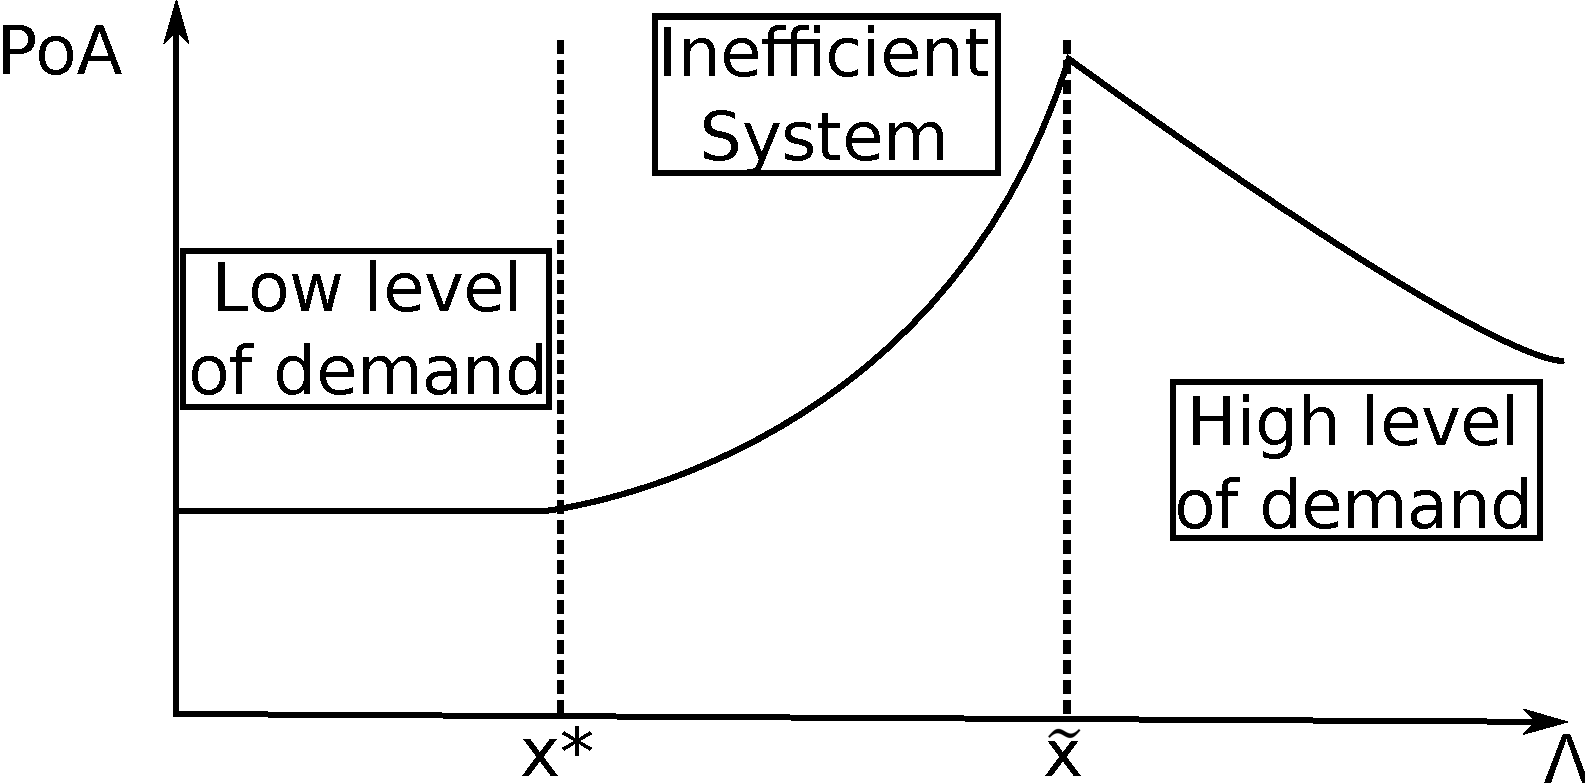
\includegraphics[width=.7\textwidth]{./Images/PoAPlotForSimpleDiagram.pdf}
\end{center}
\caption{General profile of PoA.}\label{fig:poaprofile}
\end{figure}

To consider systems where individuals are able to observe the system there are two approaches: the first is to use a simulation based approach that allows individuals to choose their most desirable queue.
One such approach that was considered specifically in the context of healthcare was considered in \cite{}.

Given that individuals will consider a simple selfish decision rule this approach is relatively straightforward and can also be considered using straightforward analytical Markov models.
The difficulty with this approach is appears when attempting to obtain the PoA.
To carry this out an optimal policy must be obtained.

In \cite{} various dynamic programming and approximate dynamic programming techniques are proposed that are able to not only give an optimal policy but also prove the following observation:

\begin{center}
\textit{Selfish users make busier systems.}
\end{center}

In the next section selfish congestion related decisions by managers will be considered.

\section{CCU Work}

The main proposition of the work requested by the ABUHB was to develop a mathematical model of bed occupancies at the CCUs at RG and NH.
After an initial analysis of the data, behavioural aspects became apparent; for example, delaying patients discharge if there was no pressure on CCU beds, or admitting fewer patients if bed occupancy levels were high.
As a result of this, a state-dependent queueing model has been developed, which includes the dependency of admission rate on actual occupancy \cite{Komenda2013}.
This state dependent model was applied to both NH and RG separately.
It is however obvious that the actions of one CCU impact on the other CCU, as diversion of patients from one CCU to the other sometimes occurs.
A pictorial representation of the situation is given in Figure \ref{diagramofdiversion}.

\begin{figure}[!htbp]
\begin{center}
\begin{tikzpicture}
\node (A) at (0,0) [draw] {RG};
\node (B) at (2,0) [draw] {NH};
\draw [->] (-1,0) -- (A);
\draw [->] (3,0) -- (B);
\draw [->] (-1,0) -- ($(A)+(-.5,0)$) -- ($(A)+(-.5,.5)$) -- ($(A)+(.5,.5)$) -- ($(A)+(.5,.1)$) -- ($(B)+(-.4,.1)$);
\draw [->] (3,0) -- ($(B)+(.5,0)$) -- ($(B)+(.5,-.5)$) -- ($(B)+(-.5,-.5)$) -- ($(B)+(-.5,-.1)$) -- ($(A)+(.4,-.1)$);
\draw [->] (3,0) -- (B);
\node at ($(A) + (0,.8)$) {Divert?};
\node at ($(B) + (0,-.8)$) {Divert?};
\end{tikzpicture}
\caption{Diagrammatic representation of CCU interaction through patient diversion.}\label{diagramofdiversion}
\end{center}
\end{figure}

The capacity thresholds are denoted as $K_{h}\in\mathbb{Z}$ for $h\in\{\NH,\RG\}$. Note that $0\leq K_h\leq c_h$.

\begin{figure}[!htbp]
\begin{center}
    \begin{tikzpicture}
        \draw  (0,0) rectangle (4,3);
        \draw [dashed, red, thick] (0,1) -- (4,1);
        \draw [dashed, red, thick] (3,0) -- (3,3);
        \node at (-.5,1) {$K_{\NH}$};
        \node at (3,3.25) {$K_{\RG}$};
        \node at (1.5,2) {$\lambda_{h}^{(a)}$};
        \node at (3.5,2) {$\lambda_{h}^{(b)}$};
        \node at (1.5,.5) {$\lambda_{h}^{(c)}$};
        \node at (3.5,.5) {$\lambda_{h}^{(d)}$};
    \end{tikzpicture}
\caption{General arrival rates for each CCU at each region, where $h\in\{\NH, \RG\}$} \label{arrivalrateregions}
\end{center}
\end{figure}

\begin{figure}[!htbp]
\begin{center}
\begin{tikzpicture}[scale=.7, every node/.style={scale=0.7}]
    % -----------------------------------------------
    % Boundaries ------------------------------------
    % -----------------------------------------------
    \draw [dashed, line width=1mm, red, opacity=.3] (12,2) -- (12,-20);
    \draw [dashed, line width=1mm, red, opacity=.3] (-2,-12) -- (20,-12);
    %\tikzstyle{state}=[ellipse, draw, fill=blue!10, minimum width=2cm];
    %\tikzstyle{state}=[rectangle, draw, fill=blue!10, minimum width=2cm];
    \tikzstyle{state}=[minimum width=2cm, font=\boldmath];
    %\draw  (0,0) rectangle (4,3);
    %\draw [dashed, red, thick] (0,1) -- (4,1);
    %\draw [dashed, red, thick] (3,0) -- (3,3);
    % -----------------------------------------------
    % First row--------------------------------------
    % -----------------------------------------------
    \node (aa) [state] at (0,0) {$(0,0)$};
    \node (ab) [state] at ($(aa) + (3,0)$) {$(0,1)$};
    \node (ac) [state] at ($(ab) + (3,0)$) {$(0,2)$};
    \node (ellipsisa1) at ($(ac) + (3,0)$) {$\dots$};
    \node(ak) [state] at ($(ellipsisa1) + (3,0)$) {$(0,K_{1})$};
    \node (ellipsisa2) at ($(ak) + (3,0)$) {$\dots$};
    \node(az) [state] at ($(ellipsisa2) + (3,0)$) {$(0,c_{1})$};
    % Transitions -----------------------------------
    % On Row:
    \draw (aa) edge[out=45,in=135,->,thick] node [above] {\tiny$\lambda_{1}^{(a)}$} (ab);
    \draw (aa) edge[out=-45,in=-135,<-,thick] node [below] {\tiny$\mu_{1}$} (ab);

    \draw (ab) edge[out=45,in=135,->,thick] node [above] {\tiny$\lambda_{1}^{(a)}$} (ac);
    \draw (ab) edge[out=-45,in=-135,<-,thick] node [below] {\tiny$\mu_{1}$} (ac);

    \draw (ac) edge[out=45,in=135,->,thick] node [above] {\tiny$\lambda_{1}^{(a)}$} (ellipsisa1);
    \draw (ac) edge[out=-45,in=-135,<-,thick] node [below] {\tiny$\mu_{1}$} (ellipsisa1);

    \draw (ellipsisa1) edge[out=45,in=135,->,thick] node [above] {\tiny$\lambda_{1}^{(a)}$} (ak);
    \draw (ellipsisa1) edge[out=-45,in=-135,<-,thick] node [below] {\tiny$\mu_{1}$} (ak);

    \draw (ak) edge[out=45,in=135,->,thick] node [above] {\tiny$\lambda_{1}^{(b)}$} (ellipsisa2);
    \draw (ak) edge[out=-45,in=-135,<-,thick] node [below] {\tiny$\mu_{1}$} (ellipsisa2);

    \draw (ellipsisa2) edge[out=45,in=135,->,thick] node [above] {\tiny$\lambda_{1}^{(b)}$} (az);
    \draw (ellipsisa2) edge[out=-45,in=-135,<-,thick] node [below] {\tiny$\mu_{1}$} (az);
    % -----------------------------------------------
    % Second row--------------------------------------
    % -----------------------------------------------
    \node (ba) [state] at (0,-3) {$(1,0)$};
    \node (bb) [state] at ($(ba) + (3,0)$) {$(1,1)$};
    \node (bc) [state] at ($(bb) + (3,0)$) {$(1,2)$};
    \node (ellipsisb1) at ($(bc) + (3,0)$) {$\dots$};
    \node(bk) [state] at ($(ellipsisb1) + (3,0)$) {$(1,K_{1})$};
    \node (ellipsisb2) at ($(bk) + (3,0)$) {$\dots$};
    \node(bz) [state] at ($(ellipsisb2) + (3,0)$) {$(1,c_{1})$};
    % Transitions -----------------------------------
    % On Row:
    \draw (ba) edge[out=45,in=135,->,thick] node [above] {\tiny$\lambda_{1}^{(a)}$} (bb);
    \draw (ba) edge[out=-45,in=-135,<-,thick] node [below] {\tiny$\mu_{1}$} (bb);

    \draw (bb) edge[out=45,in=135,->,thick] node [above] {\tiny$\lambda_{1}^{(a)}$} (bc);
    \draw (bb) edge[out=-45,in=-135,<-,thick] node [below] {\tiny$\mu_{1}$} (bc);

    \draw (bc) edge[out=45,in=135,->,thick] node [above] {\tiny$\lambda_{1}^{(a)}$} (ellipsisb1);
    \draw (bc) edge[out=-45,in=-135,<-,thick] node [below] {\tiny$\mu_{1}$} (ellipsisb1);

    \draw (ellipsisb1) edge[out=45,in=135,->,thick] node [above] {\tiny$\lambda_{1}^{(a)}$} (bk);
    \draw (ellipsisb1) edge[out=-45,in=-135,<-,thick] node [below] {\tiny$\mu_{1}$} (bk);

    \draw (bk) edge[out=45,in=135,->,thick] node [above] {\tiny$\lambda_{1}^{(b)}$} (ellipsisb2);
    \draw (bk) edge[out=-45,in=-135,<-,thick] node [below] {\tiny$\mu_{1}$} (ellipsisb2);

    \draw (ellipsisb2) edge[out=45,in=135,->,thick] node [above] {\tiny$\lambda_{1}^{(b)}$} (bz);
    \draw (ellipsisb2) edge[out=-45,in=-135,<-,thick] node [below] {\tiny$\mu_{1}$} (bz);
    % With previous row:
    \draw (aa) edge[out=-125,in=125,->,thick] node [left] {\tiny$\lambda_{2}^{(a)}$} (ba);
    \draw (aa) edge[out=-55,in=55,<-,thick] node [right] {\tiny$\mu_{2}$} (ba);

    \draw (ab) edge[out=-125,in=125,->,thick] node [left] {\tiny$\lambda_{2}^{(a)}$} (bb);
    \draw (ab) edge[out=-55,in=55,<-,thick] node [right] {\tiny$\mu_{2}$} (bb);

    \draw (ac) edge[out=-125,in=125,->,thick] node [left] {\tiny$\lambda_{2}^{(a)}$} (bc);
    \draw (ac) edge[out=-55,in=55,<-,thick] node [right] {\tiny$\mu_{2}$} (bc);

    \draw (ellipsisa1) edge[out=-125,in=125,->,thick] node [left] {\tiny$\lambda_{2}^{(a)}$} (ellipsisb1);
    \draw (ellipsisa1) edge[out=-55,in=55,<-,thick] node [right] {\tiny$\mu_{2}$} (ellipsisb1);

    \draw (ak) edge[out=-125,in=125,->,thick] node [left] {\tiny$\lambda_{2}^{(b)}$} (bk);
    \draw (ak) edge[out=-55,in=55,<-,thick] node [right] {\tiny$\mu_{2}$} (bk);

    \draw (ellipsisa2) edge[out=-125,in=125,->,thick] node [left] {\tiny$\lambda_{2}^{(b)}$} (ellipsisb2);
    \draw (ellipsisa2) edge[out=-55,in=55,<-,thick] node [right] {\tiny$\mu_{2}$} (ellipsisb2);

    \draw (az) edge[out=-125,in=125,->,thick] node [left] {\tiny$\lambda_{2}^{(b)}$} (bz);
    \draw (az) edge[out=-55,in=55,<-,thick] node [right] {\tiny$\mu_{2}$} (bz);
    % -----------------------------------------------
    % Third row--------------------------------------
    % -----------------------------------------------
    \node (ca) [state] at (0,-6) {$(2,0)$};
    \node (cb) [state] at ($(ca) + (3,0)$) {$(2,1)$};
    \node (cc) [state] at ($(cb) + (3,0)$) {$(2,2)$};
    \node (ellipsisc1) at ($(cc) + (3,0)$) {$\dots$};
    \node(ck) [state] at ($(ellipsisc1) + (3,0)$) {$(2,K_{1})$};
    \node (ellipsisc2) at ($(ck) + (3,0)$) {$\dots$};
    \node(cz) [state] at ($(ellipsisc2) + (3,0)$) {$(2,c_{1})$};
    % Transitions -----------------------------------
    % On Row:
    \draw (ca) edge[out=45,in=135,->,thick] node [above] {\tiny$\lambda_{1}^{(a)}$} (cb);
    \draw (ca) edge[out=-45,in=-135,<-,thick] node [below] {\tiny$\mu_{1}$} (cb);

    \draw (cb) edge[out=45,in=135,->,thick] node [above] {\tiny$\lambda_{1}^{(a)}$} (cc);
    \draw (cb) edge[out=-45,in=-135,<-,thick] node [below] {\tiny$\mu_{1}$} (cc);

    \draw (cc) edge[out=45,in=135,->,thick] node [above] {\tiny$\lambda_{1}^{(a)}$} (ellipsisc1);
    \draw (cc) edge[out=-45,in=-135,<-,thick] node [below] {\tiny$\mu_{1}$} (ellipsisc1);

    \draw (ellipsisc1) edge[out=45,in=135,->,thick] node [above] {\tiny$\lambda_{1}^{(a)}$} (ck);
    \draw (ellipsisc1) edge[out=-45,in=-135,<-,thick] node [below] {\tiny$\mu_{1}$} (ck);

    \draw (ck) edge[out=45,in=135,->,thick] node [above] {\tiny$\lambda_{1}^{(b)}$} (ellipsisc2);
    \draw (ck) edge[out=-45,in=-135,<-,thick] node [below] {\tiny$\mu_{1}$} (ellipsisc2);

    \draw (ellipsisc2) edge[out=45,in=135,->,thick] node [above] {\tiny$\lambda_{1}^{(b)}$} (cz);
    \draw (ellipsisc2) edge[out=-45,in=-135,<-,thick] node [below] {\tiny$\mu_{1}$} (cz);
    % With previous row:
    \draw (ba) edge[out=-125,in=125,->,thick] node [left] {\tiny$\lambda_{2}^{(a)}$} (ca);
    \draw (ba) edge[out=-55,in=55,<-,thick] node [right] {\tiny$\mu_{2}$} (ca);

    \draw (bb) edge[out=-125,in=125,->,thick] node [left] {\tiny$\lambda_{2}^{(a)}$} (cb);
    \draw (bb) edge[out=-55,in=55,<-,thick] node [right] {\tiny$\mu_{2}$} (cb);

    \draw (bc) edge[out=-125,in=125,->,thick] node [left] {\tiny$\lambda_{2}^{(a)}$} (cc);
    \draw (bc) edge[out=-55,in=55,<-,thick] node [right] {\tiny$\mu_{2}$} (cc);

    \draw (ellipsisb1) edge[out=-125,in=125,->,thick] node [left] {\tiny$\lambda_{2}^{(a)}$} (ellipsisc1);
    \draw (ellipsisb1) edge[out=-55,in=55,<-,thick] node [right] {\tiny$\mu_{2}$} (ellipsisc1);

    \draw (bk) edge[out=-125,in=125,->,thick] node [left] {\tiny$\lambda_{2}^{(b)}$} (ck);
    \draw (bk) edge[out=-55,in=55,<-,thick] node [right] {\tiny$\mu_{2}$} (ck);

    \draw (ellipsisb2) edge[out=-125,in=125,->,thick] node [left] {\tiny$\lambda_{2}^{(b)}$} (ellipsisc2);
    \draw (ellipsisb2) edge[out=-55,in=55,<-,thick] node [right] {\tiny$\mu_{2}$} (ellipsisc2);

    \draw (bz) edge[out=-125,in=125,->,thick] node [left] {\tiny$\lambda_{2}^{(b)}$} (cz);
    \draw (bz) edge[out=-55,in=55,<-,thick] node [right] {\tiny$\mu_{2}$} (cz);
    % -----------------------------------------------
    % Fourth row--------------------------------------
    % -----------------------------------------------
    \node (da) at (0,-9) {$\vdots$};
    \node (db) at ($(da) + (3,0)$) {$\vdots$};
    \node (dc) at ($(db) + (3,0)$) {$\vdots$};
    \node (ellipsisd1) at ($(dc) + (3,0)$) {$\dots$};
    \node(dk) at ($(ellipsisd1) + (3,0)$) {$\vdots$};
    \node (ellipsisd2) at ($(dk) + (3,0)$) {$\dots$};
    \node(dz) at ($(ellipsisd2) + (3,0)$) {$\vdots$};
    % Transitions -----------------------------------
    % On Row:
    \draw (da) edge[out=45,in=135,->,thick] node [above] {\tiny$\lambda_{1}^{(a)}$} (db);
    \draw (da) edge[out=-45,in=-135,<-,thick] node [below] {\tiny$\mu_{1}$} (db);

    \draw (db) edge[out=45,in=135,->,thick] node [above] {\tiny$\lambda_{1}^{(a)}$} (dc);
    \draw (db) edge[out=-45,in=-135,<-,thick] node [below] {\tiny$\mu_{1}$} (dc);

    \draw (dc) edge[out=45,in=135,->,thick] node [above] {\tiny$\lambda_{1}^{(a)}$} (ellipsisd1);
    \draw (dc) edge[out=-45,in=-135,<-,thick] node [below] {\tiny$\mu_{1}$} (ellipsisd1);

    \draw (ellipsisd1) edge[out=45,in=135,->,thick] node [above] {\tiny$\lambda_{1}^{(a)}$} (dk);
    \draw (ellipsisd1) edge[out=-45,in=-135,<-,thick] node [below] {\tiny$\mu_{1}$} (dk);

    \draw (dk) edge[out=45,in=135,->,thick] node [above] {\tiny$\lambda_{1}^{(b)}$} (ellipsisd2);
    \draw (dk) edge[out=-45,in=-135,<-,thick] node [below] {\tiny$\mu_{1}$} (ellipsisd2);

    \draw (ellipsisd2) edge[out=45,in=135,->,thick] node [above] {\tiny$\lambda_{1}^{(b)}$} (dz);
    \draw (ellipsisd2) edge[out=-45,in=-135,<-,thick] node [below] {\tiny$\mu_{1}$} (dz);
    % With previous row:
    \draw (ca) edge[out=-125,in=125,->,thick] node [left] {\tiny$\lambda_{2}^{(a)}$} (da);
    \draw (ca) edge[out=-55,in=55,<-,thick] node [right] {\tiny$\mu_{2}$} (da);

    \draw (cb) edge[out=-125,in=125,->,thick] node [left] {\tiny$\lambda_{2}^{(a)}$} (db);
    \draw (cb) edge[out=-55,in=55,<-,thick] node [right] {\tiny$\mu_{2}$} (db);

    \draw (cc) edge[out=-125,in=125,->,thick] node [left] {\tiny$\lambda_{2}^{(a)}$} (dc);
    \draw (cc) edge[out=-55,in=55,<-,thick] node [right] {\tiny$\mu_{2}$} (dc);

    \draw (ellipsisc1) edge[out=-125,in=125,->,thick] node [left] {\tiny$\lambda_{2}^{(a)}$} (ellipsisd1);
    \draw (ellipsisc1) edge[out=-55,in=55,<-,thick] node [right] {\tiny$\mu_{2}$} (ellipsisd1);

    \draw (ck) edge[out=-125,in=125,->,thick] node [left] {\tiny$\lambda_{2}^{(b)}$} (dk);
    \draw (ck) edge[out=-55,in=55,<-,thick] node [right] {\tiny$\mu_{2}$} (dk);

    \draw (ellipsisc2) edge[out=-125,in=125,->,thick] node [left] {\tiny$\lambda_{2}^{(b)}$} (ellipsisd2);
    \draw (ellipsisc2) edge[out=-55,in=55,<-,thick] node [right] {\tiny$\mu_{2}$} (ellipsisd2);

    \draw (cz) edge[out=-125,in=125,->,thick] node [left] {\tiny$\lambda_{2}^{(b)}$} (dz);
    \draw (cz) edge[out=-55,in=55,<-,thick] node [right] {\tiny$\mu_{2}$} (dz);
    % -----------------------------------------------
    % Fifth row--------------------------------------
    % -----------------------------------------------
    \node (ea) [state] at (0,-12) {$(K_{2},0)$};
    \node (eb) [state] at ($(ea) + (3,0)$) {$(K_{2},1)$};
    \node (ec) [state] at ($(eb) + (3,0)$) {$(K_{2},2)$};
    \node (ellipsise1) at ($(ec) + (3,0)$) {$\dots$};
    \node(ek) [state] at ($(ellipsise1) + (3,0)$) {$(K_{2},K_{1})$};
    \node (ellipsise2) at ($(ek) + (3,0)$) {$\dots$};
    \node(ez) [state] at ($(ellipsise2) + (3,0)$) {$(K_{2},c_{1})$};
    % Transitions -----------------------------------
    % On Row:
    \draw (ea) edge[out=45,in=135,->,thick] node [above] {\tiny$\lambda_{1}^{(c)}$} (eb);
    \draw (ea) edge[out=-45,in=-135,<-,thick] node [below] {\tiny$\mu_{1}$} (eb);

    \draw (eb) edge[out=45,in=135,->,thick] node [above] {\tiny$\lambda_{1}^{(c)}$} (ec);
    \draw (eb) edge[out=-45,in=-135,<-,thick] node [below] {\tiny$\mu_{1}$} (ec);

    \draw (ec) edge[out=45,in=135,->,thick] node [above] {\tiny$\lambda_{1}^{(c)}$} (ellipsise1);
    \draw (ec) edge[out=-45,in=-135,<-,thick] node [below] {\tiny$\mu_{1}$} (ellipsise1);

    \draw (ellipsise1) edge[out=45,in=135,->,thick] node [above] {\tiny$\lambda_{1}^{(c)}$} (ek);
    \draw (ellipsise1) edge[out=-45,in=-135,<-,thick] node [below] {\tiny$\mu_{1}$} (ek);

    \draw (ek) edge[out=45,in=135,->,thick] node [above] {\tiny$\lambda_{1}^{(d)}$} (ellipsise2);
    \draw (ek) edge[out=-45,in=-135,<-,thick] node [below] {\tiny$\mu_{1}$} (ellipsise2);

    \draw (ellipsise2) edge[out=45,in=135,->,thick] node [above] {\tiny$\lambda_{1}^{(d)}$} (ez);
    \draw (ellipsise2) edge[out=-45,in=-135,<-,thick] node [below] {\tiny$\mu_{1}$} (ez);
    % With previous row:
    \draw (da) edge[out=-125,in=125,->,thick] node [left] {\tiny$\lambda_{2}^{(a)}$} (ea);
    \draw (da) edge[out=-55,in=55,<-,thick] node [right] {\tiny$\mu_{2}$} (ea);

    \draw (db) edge[out=-125,in=125,->,thick] node [left] {\tiny$\lambda_{2}^{(a)}$} (eb);
    \draw (db) edge[out=-55,in=55,<-,thick] node [right] {\tiny$\mu_{2}$} (eb);

    \draw (dc) edge[out=-125,in=125,->,thick] node [left] {\tiny$\lambda_{2}^{(a)}$} (ec);
    \draw (dc) edge[out=-55,in=55,<-,thick] node [right] {\tiny$\mu_{2}$} (ec);

    \draw (ellipsisd1) edge[out=-125,in=125,->,thick] node [left] {\tiny$\lambda_{2}^{(a)}$} (ellipsise1);
    \draw (ellipsisd1) edge[out=-55,in=55,<-,thick] node [right] {\tiny$\mu_{2}$} (ellipsise1);

    \draw (dk) edge[out=-125,in=125,->,thick] node [left] {\tiny$\lambda_{2}^{(b)}$} (ek);
    \draw (dk) edge[out=-55,in=55,<-,thick] node [right] {\tiny$\mu_{2}$} (ek);

    \draw (ellipsisd2) edge[out=-125,in=125,->,thick] node [left] {\tiny$\lambda_{2}^{(b)}$} (ellipsise2);
    \draw (ellipsisd2) edge[out=-55,in=55,<-,thick] node [right] {\tiny$\mu_{2}$} (ellipsise2);

    \draw (dz) edge[out=-125,in=125,->,thick] node [left] {\tiny$\lambda_{2}^{(b)}$} (ez);
    \draw (dz) edge[out=-55,in=55,<-,thick] node [right] {\tiny$\mu_{2}$} (ez);
    % Sixth row--------------------------------------
    \node (fa) at (0,-15) {$\vdots$};
    \node (fb) at ($(fa) + (3,0)$) {$\vdots$};
    \node (fc) at ($(fb) + (3,0)$) {$\vdots$};
    \node (ellipsisf1) at ($(fc) + (3,0)$) {$\dots$};
    \node(fk) at ($(ellipsisf1) + (3,0)$) {$\vdots$};
    \node (ellipsisf2) at ($(fk) + (3,0)$) {$\dots$};
    \node(fz) at ($(ellipsisf2) + (3,0)$) {$\vdots$};
    % Transitions -----------------------------------
    % On Row:
    \draw (fa) edge[out=45,in=135,->,thick] node [above] {\tiny$\lambda_{1}^{(c)}$} (fb);
    \draw (fa) edge[out=-45,in=-135,<-,thick] node [below] {\tiny$\mu_{1}$} (fb);

    \draw (fb) edge[out=45,in=135,->,thick] node [above] {\tiny$\lambda_{1}^{(c)}$} (fc);
    \draw (fb) edge[out=-45,in=-135,<-,thick] node [below] {\tiny$\mu_{1}$} (fc);

    \draw (fc) edge[out=45,in=135,->,thick] node [above] {\tiny$\lambda_{1}^{(c)}$} (ellipsisf1);
    \draw (fc) edge[out=-45,in=-135,<-,thick] node [below] {\tiny$\mu_{1}$} (ellipsisf1);

    \draw (ellipsisf1) edge[out=45,in=135,->,thick] node [above] {\tiny$\lambda_{1}^{(c)}$} (fk);
    \draw (ellipsisf1) edge[out=-45,in=-135,<-,thick] node [below] {\tiny$\mu_{1}$} (fk);

    \draw (fk) edge[out=45,in=135,->,thick] node [above] {\tiny$\lambda_{1}^{(d)}$} (ellipsisf2);
    \draw (fk) edge[out=-45,in=-135,<-,thick] node [below] {\tiny$\mu_{1}$} (ellipsisf2);

    \draw (ellipsisf2) edge[out=45,in=135,->,thick] node [above] {\tiny$\lambda_{1}^{(d)}$} (fz);
    \draw (ellipsisf2) edge[out=-45,in=-135,<-,thick] node [below] {\tiny$\mu_{1}$} (fz);
    % With previous row:
    \draw (ea) edge[out=-125,in=125,->,thick] node [left] {\tiny$\lambda_{2}^{(c)}$} (fa);
    \draw (ea) edge[out=-55,in=55,<-,thick] node [right] {\tiny$\mu_{2}$} (fa);

    \draw (eb) edge[out=-125,in=125,->,thick] node [left] {\tiny$\lambda_{2}^{(c)}$} (fb);
    \draw (eb) edge[out=-55,in=55,<-,thick] node [right] {\tiny$\mu_{2}$} (fb);

    \draw (ec) edge[out=-125,in=125,->,thick] node [left] {\tiny$\lambda_{2}^{(c)}$} (fc);
    \draw (ec) edge[out=-55,in=55,<-,thick] node [right] {\tiny$\mu_{2}$} (fc);

    \draw (ellipsise1) edge[out=-125,in=125,->,thick] node [left] {\tiny$\lambda_{2}^{(c)}$} (ellipsisf1);
    \draw (ellipsise1) edge[out=-55,in=55,<-,thick] node [right] {\tiny$\mu_{2}$} (ellipsisf1);

    \draw (ek) edge[out=-125,in=125,->,thick] node [left] {\tiny$\lambda_{2}^{(d)}$} (fk);
    \draw (ek) edge[out=-55,in=55,<-,thick] node [right] {\tiny$\mu_{2}$} (fk);

    \draw (ellipsise2) edge[out=-125,in=125,->,thick] node [left] {\tiny$\lambda_{2}^{(d)}$} (ellipsisf2);
    \draw (ellipsise2) edge[out=-55,in=55,<-,thick] node [right] {\tiny$\mu_{2}$} (ellipsisf2);

    \draw (ez) edge[out=-125,in=125,->,thick] node [left] {\tiny$\lambda_{2}^{(d)}$} (fz);
    \draw (ez) edge[out=-55,in=55,<-,thick] node [right] {\tiny$\mu_{2}$} (fz);
    % Final row--------------------------------------
    \node (za) [state] at (0,-18) {$(c_{2},0)$};
    \node (zb) [state] at ($(za) + (3,0)$) {$(c_{2},1)$};
    \node (zc) [state] at ($(zb) + (3,0)$) {$(c_{2},2)$};
    \node (ellipsisz1) at ($(zc) + (3,0)$) {$\dots$};
    \node(zk) [state] at ($(ellipsisz1) + (3,0)$) {$(c_{2},K_{1})$};
    \node (ellipsisz2) at ($(zk) + (3,0)$) {$\dots$};
    \node(zz) [state] at ($(ellipsisz2) + (3,0)$) {$(c_{2},c_{1})$};
    % Transitions -----------------------------------
    % On Row:
    \draw (za) edge[out=45,in=135,->,thick] node [above] {\tiny$\lambda_{1}^{(d)}$} (zb);
    \draw (za) edge[out=-45,in=-135,<-,thick] node [below] {\tiny$\mu_{1}$} (zb);

    \draw (zb) edge[out=45,in=135,->,thick] node [above] {\tiny$\lambda_{1}^{(d)}$} (zc);
    \draw (zb) edge[out=-45,in=-135,<-,thick] node [below] {\tiny$\mu_{1}$} (zc);

    \draw (zc) edge[out=45,in=135,->,thick] node [above] {\tiny$\lambda_{1}^{(d)}$} (ellipsisz1);
    \draw (zc) edge[out=-45,in=-135,<-,thick] node [below] {\tiny$\mu_{1}$} (ellipsisz1);

    \draw (ellipsisz1) edge[out=45,in=135,->,thick] node [above] {\tiny$\lambda_{1}^{(d)}$} (zk);
    \draw (ellipsisz1) edge[out=-45,in=-135,<-,thick] node [below] {\tiny$\mu_{1}$} (zk);

    \draw (zk) edge[out=45,in=135,->,thick] node [above] {\tiny$\lambda_{1}^{(d)}$} (ellipsisz2);
    \draw (zk) edge[out=-45,in=-135,<-,thick] node [below] {\tiny$\mu_{1}$} (ellipsisz2);

    \draw (ellipsisz2) edge[out=45,in=135,->,thick] node [above] {\tiny$\lambda_{1}^{(d)}$} (zz);
    \draw (ellipsisz2) edge[out=-45,in=-135,<-,thick] node [below] {\tiny$\mu_{1}$} (zz);
    % With previous row:
    \draw (fa) edge[out=-125,in=125,->,thick] node [left] {\tiny$\lambda_{2}^{(c)}$} (za);
    \draw (fa) edge[out=-55,in=55,<-,thick] node [right] {\tiny$\mu_{2}$} (za);

    \draw (fb) edge[out=-125,in=125,->,thick] node [left] {\tiny$\lambda_{2}^{(c)}$} (zb);
    \draw (fb) edge[out=-55,in=55,<-,thick] node [right] {\tiny$\mu_{2}$} (zb);

    \draw (fc) edge[out=-125,in=125,->,thick] node [left] {\tiny$\lambda_{2}^{(c)}$} (zc);
    \draw (fc) edge[out=-55,in=55,<-,thick] node [right] {\tiny$\mu_{2}$} (zc);

    \draw (ellipsisf1) edge[out=-125,in=125,->,thick] node [left] {\tiny$\lambda_{2}^{(c)}$} (ellipsisz1);
    \draw (ellipsisf1) edge[out=-55,in=55,<-,thick] node [right] {\tiny$\mu_{2}$} (ellipsisz1);

    \draw (fk) edge[out=-125,in=125,->,thick] node [left] {\tiny$\lambda_{2}^{(d)}$} (zk);
    \draw (fk) edge[out=-55,in=55,<-,thick] node [right] {\tiny$\mu_{2}$} (zk);

    \draw (ellipsisf2) edge[out=-125,in=125,->,thick] node [left] {\tiny$\lambda_{2}^{(d)}$} (ellipsisz2);
    \draw (ellipsisf2) edge[out=-55,in=55,<-,thick] node [right] {\tiny$\mu_{2}$} (ellipsisz2);

    \draw (fz) edge[out=-125,in=125,->,thick] node [left] {\tiny$\lambda_{2}^{(d)}$} (zz);
    \draw (fz) edge[out=-55,in=55,<-,thick] node [right] {\tiny$\mu_{2}$} (zz);

\end{tikzpicture}

\caption{Generic Markov chain underpinning the queueing model of this paper} \label{mc}
\end{center}
\end{figure}

Utilities will be of interest when this queueing theoretical model will be inserted in the game theoretical model.
Throughput of patients is a natural choice of utility given that most hospitals are financially rewarded per served patient \cite{Pate2009}.
For each threshold pair $(K_{\NH},K_{\RG})$, the utilisation rate $U_h$ and throughput $T_h$ can easily be obtained for each CCU: $h\in\{\text{NH},\text{RG}\}$, using the following formulas:

$$U_{h}={{\sum_{n=0}^{c_h} nP^{(h)}(n)}\over{c_{h}}}$$
$$T_{h}=\mu_h \sum _{n=0}^{c_h} nP^{(h)}(n)$$

where $P^{(h)}=P^{(h)}(K_{\NH},K_{\RG})$ is the steady state probability distribution function (obtained from the corresponding transition matrix $Q=Q(K_{\NH},K_{\RG})$) for $h\in\{\text{NH},\text{RG}\}$.

For $c_{\NH}=8$, $c_{\RG}=16$, $\lambda_{\NH}=(\lambda_{\NH}^{(a)},\lambda_{\NH}^{(b)},\lambda_{\NH}^{(c)},\lambda_{\NH}^{(d)})=(1.5,3.74,0,0)$, $\lambda_{\RG}=(\lambda_{\RG}^{(a)},\lambda_{\RG}^{(b)},\lambda_{\RG}^{(c)},\lambda_{\RG}^{(d)})=(2.24,0,3.74,0)$ and $(K_{\NH},K_{\RG})=(6,12)$, the steady state probabilities for each CCU are given in Figure \ref{steady_state_probs}.


\begin{figure}[!htbp]
\hspace{2cm}For all $h\in\{\text{NH}, \text{RG}\}$ minimise:
$$\left(U_{h}-t\right)^2$$
\hspace{2cm}Subject to:
\begin{align}
0\leq & K_h \leq c_{h}\nonumber\\
&K_h \in  \mathbb{Z}\nonumber
\end{align}
\caption{The optimisation problem underlying the game}\label{model1}
\end{figure}

This game is equivalent to a bi matrix game with restriction to pure strategies where both players aim to get their utilisation as close as possible to a certain target.
As such a Nash Equilibrium is not guaranteed by traditional game theoretical results \cite{Nash1950}, but based on discussions with ABUHB, long term threshold policies are a realistic consideration.

The following result is a sufficient condition for the existence of an equilibrium:\\


\textbf{Theorem.}

Let $f_{h}(k):[1,c_{\bar h}]\to[1,c_h]$ be the best response of player $h\in\{\NH, \RG\}$ to the diversion threshold of $\bar h\ne h$ ($\bar h\in\{\NH, \RG\}$).

If $f_{h}(k)$ is a non-decreasing function in $k$ then the game of Figure \ref{model1} has at least one Nash Equilibrium.


\textbf{proof}

The function $f_h$ is well defined as it maximises a continuous function over a finite discrete set (in case of multiple values that minimize $U_h$, it is assumed that $f_h$ returns the lowest such value).

As such if $f_h$ is non-decreasing then it is in fact a stepwise non-decreasing function.
If we consider $f_{\NH}$ and $f_{\RG}$ plotted on the same axis (so that the domain of $f_{\NH}$ is the $x$-axis and the domain of $f_{\RG}$ is the y-axis) it is obvious to see that the functions must intersect at some point as shown in Figure \ref{exampleforproof}.

\begin{figure}[!htbp]
$$\begin{array}{cc}
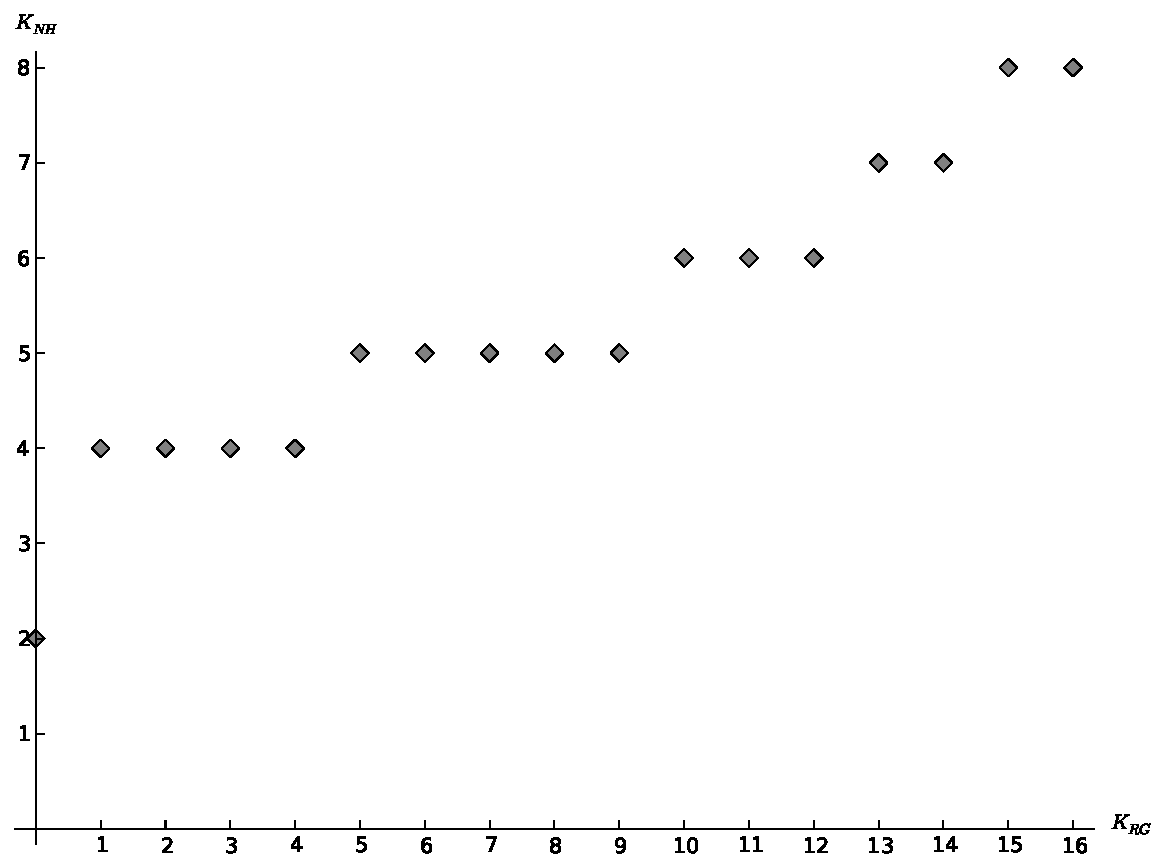
\includegraphics[width=.5\textwidth]{./Images/best_responses_ex_for_proof_NH.pdf}&
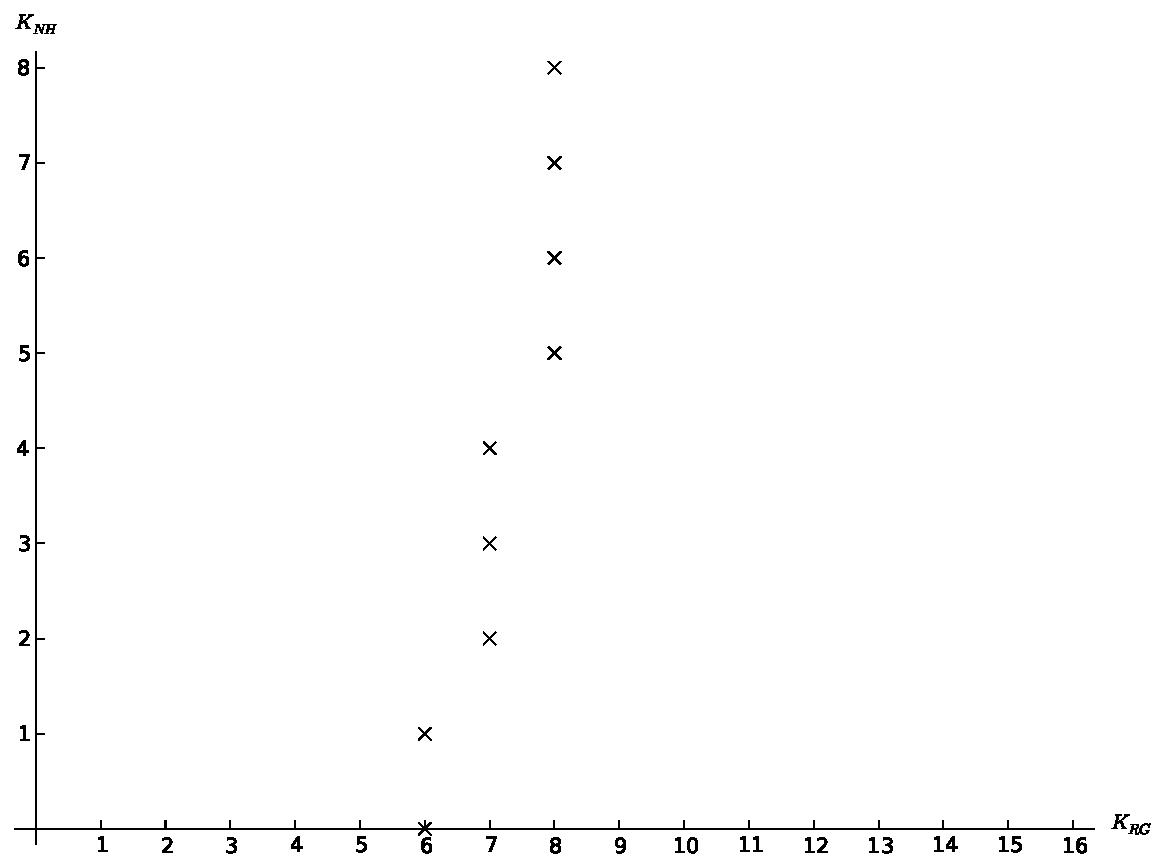
\includegraphics[width=.5\textwidth]{./Images/best_responses_ex_for_proof_RG.pdf}
\end{array}$$
\caption{Plots of $f_{\NH}(K_{\RG})$ and $f_{\RG}(K_{\NH})$}\label{exampleforproof}
\end{figure}

This point of intersection corresponds to a Nash Equilibrium of Figure \ref{model1}.
$\square$


\begin{figure}[!htbp]
\begin{center}
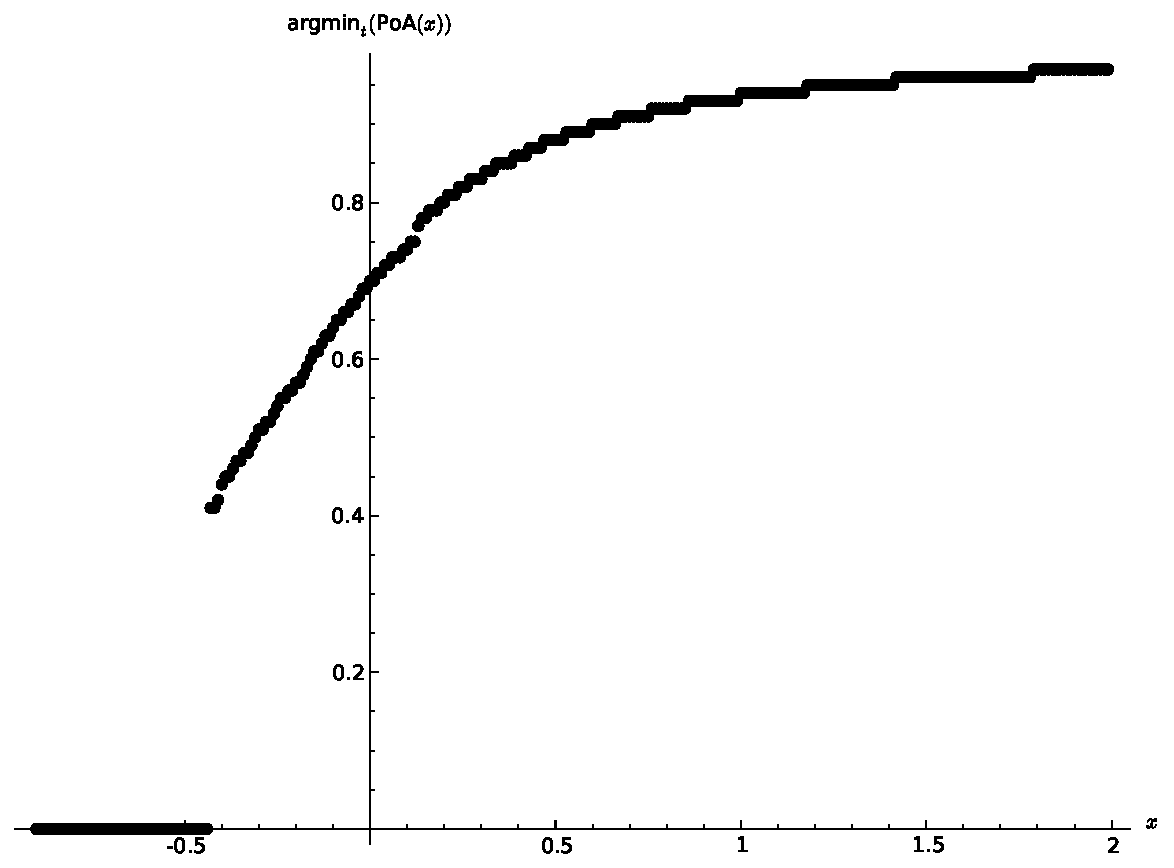
\includegraphics[width=12cm]{./Images/argminPoAmodel2.pdf}
\caption{Lowest value of $t$ ensuring PoA$=1$} \label{mintargetvdemandmodel2}
\end{center}
\end{figure}

\section{Conclusions}

\begin{itemize}
    \item Describe potential
    \item Describe further work
    \item Discuss potential for heuristic approaches
\end{itemize}

\newpage
\bibliographystyle{plain}
\bibliography{library.bib}

%\bigskip
%\noindent{\bf Refer\^encias}
%
%\noindent \textbf {Anna, A.} (1996), Comunica\c c\~ao, \textit{Atas do XXVIII SBPO}, 123-134.
%
%\noindent \textbf{Gates, B.}, \textit{Um Livro Muito Bom}, Editor, Local, 2003.
%
%\noindent  \textbf{Pel\'e, E. N. e Rom\'ario, R. R.}, Exemplo de artigo em livro, em Windows, P. T. e Linux, V. G. (Eds.),
%\textit{Colet\^ania de Artigos},  Editor, Local, 123-133, 2004.
%
%\noindent  \textbf{Silva, A. B., Souza, C. D. e Santos, E. F.}, T\'\i tulo de um relat\'orio t\'ecnico dispon\'\i vel na Internet,
%\textit{ Relat\'orios de Pesquisa em Engenharia de Produ\c c\~ao}, n. 4,  Universidade Z,
%1999
%
%\noindent{(www.universidade.br/rel, 4, 2001.}
%
%\noindent  \textbf{Smith, S. e Jones, J.} (2002), A paper on Operations Research, \textit{Pesquisa Operacional},
%32, 5-44.

\end{document}
